% Guia para a sintaxe simbólica do Matlab
\documentclass[12pt]{article}

\usepackage[utf8]{inputenc}
\usepackage[portuguese]{babel}
\usepackage{indentfirst}
\usepackage{mathtools}
\usepackage{datetime}
\usepackage{hyperref}
\usepackage{graphicx}

\author{Alice Fontes\\Camyla Tsukuda Romão\\Paulo Oliveira Lenzi Valente}

\newdateformat{mydate}{\monthname[\THEMONTH] \THEYEAR}
\date{Dezembro/2016}
\title{Relatório - Simulador de Circuitos Elétricos}

\begin{document}

\maketitle

\pagebreak
\tableofcontents
\pagebreak
\addcontentsline{toc}{section}{Introdução}
\section*{Introdução}
  Este trabalho visa a construção de um programa que analisa circuitos no domínio do tempo, utilizando análise nodal modificada e o método dos trapézios junto com o método de Newton-Raphson.

	O programa analisa circuitos compostos pelos seguintes elementos: resistores, capacitores, indutores, fontes de corrente e de tensão independentes, os quatro tipos de fontes controladas, amplificadores operacionais ideais de 4 terminais, transformadores ideais, diodos ideais e chaves ideais controladas por tensão.

\section{Funcionamento básico do simulador}
  Para utilizar o simulador, pode-se executar o programa diretamente. Nesse caso, o programa pedirá um arquivo de netlist no formato SPICE. Além disso, em ambiente Windows, pode-se executar o programa “arrastando” um arquivo de netlist “para cima” do executável. Nesse caso, o programa analisa o arquivo dado. Do mesmo modo, aceita um argumento de linha de comando, que será utilizado como nome de arquivo para analisar.

	Primeiramente, o programa faz a leitura do netlist, separando os componentes em três categorias: componentes fixos, componentes variantes e componentes não-lineares. A cada categoria corresponde uma lista de objetos que guardam a informação necessária para a simulação.

	Após a leitura do netlist, começam a ser criadas as variáveis correspondentes aos componentes fixos, como é o caso de resistores, transformadores e amp-ops. Então, programa executa uma análise de ponto de operação, também utilizada para simulação DC.

Feito isso, caso tenha sido escolhido o método de simulação TRAP, na linha .TRAN do netlist, descrita na seção seguinte, é feita a análise no tempo através do método dos trapézios. Por fim, os resultados são escritos em um arquivo de texto, no qual a primeira linha especifica a variável correspondente a cada coluna e as demais linhas, os valores. As colunas são separadas por espaços.

\section{Formato do Netlist}
O netlist do circuito a ser analisado contém uma linha de título, além dos seguintes elementos:

\begin{itemize}
  \item Especificação de análise transiente:
    .TRAN $<$tempo final$>$ $<$passo$>$ $<$método$>$ $<$passos por ponto$>$
  \item Comentários: $*<$comentário$>$
  \item Indutor: L$<$nome$>$ $<$valor$>$
  \item Resistor: R$<$nome$>$ $<$valor$>$
  \item Capacitor: C$<$nome$>$ $<$valor$>$
  \item Fontes controladas: $<$Tipo da fonte$>$$<$nome$>$ $<$saída$+>$ $<$saída$->$ $<$entrada$+>$ $<$entrada$->$
  \begin{itemize}
    \item Fonte de tensão controlada a tensão: E
    \item Fonte de corrente controlada a corrente: F
    \item Fonte de corrente controlada a tensão: G
    \item Fonte de tensão controlada a corrente: H
  \end{itemize}
  \item Fonte de corrente: I$<$nome$>$ $<$nó a$>$ $<$nó b$>$ $<$valor$>$
  \item Fonte de tensão: V$<$nome$>$ $<$nó a$>$ $<$nó b$>$ $<$valor$>$
  \item Amplificador operacional ideal: O$<$nome$>$ $<$saída$+>$ $<$saída$->$ $<$entrada$+>$ $<$entrada$->$
  \item Diodo ideal: D$<$nome$>$ $<$nó a$>$ $<$nó b$>$
  \item Chave ideal: \$$<$nome$>$ $<$nó a$>$ $<$nó b$>$ $<$nó controle$+>$ $<$nó controle$->$ $<$Vlimite$>$
  \item Transformador ideal: K$<$nome$>$ $<$nó in$+>$ $<$nó in$->$ $<$nó out$+>$ $<$nó out$->$ $<$ganho$>$
\end{itemize}


\section{Entendimento detalhado do programa}
	Para o funcionamento do programa, utilizamos as funções citadas abaixo, seguidas da explicação de seu funcionamento:\\

  \textbf{resolverSistema}

  Função para a resolução de sistema de equações lineares. Utiliza o método de Gauss-Jordan com condensação pivotal.\\

  \textbf{numero}

  Rotina que conta os nós do sistema a ser resolvido e atribui números a eles.\\

  \textbf{leituraNetlist}

  Realiza a leitura da netlist entregue e organiza as informações para a posterior resolução do sistema.\\

  \textbf{adicionarVariaveis}

  Define variáveis adicionais relativas às correntes que precisam ser calculadas no sistema.\\

  \textbf{listarVariaveis}

  Expõe as variáveis, relacionando seus nomes aos seus números no sistema.\\

  \textbf{mostrarNetlist}

  Organiza a netlist com os dados e as variáveis do sistema.\\

  \textbf{montarSistemaDC}

  Nesta função, identificamos os tipos dos elementos e montamos as estampas para cada elemento linear do sistema que não varia com o tempo, combinando-as.\\

  \textbf{mostrarSistema}

  Função opcional: Mostra o sistema resolvido.\\

  \textbf{adicionarEstampasComponentesVariantes}

  Adiciona as estampas para cada um dos componentes com estampas que variam no tempo presentes no sistema.\\

  \textbf{resolverNewtonRaphson}

  Função que executa o algoritmo de Newton Raphson para resolução do circuito, adicionando as estampas dos componentes não lineares antes de resolver o sistema.\\

  \textbf{simulacaoTrapezios}

  Esta função monta o sistema DC. A cada iteração, adiciona estampas dos componentes variantes no tempo, resolve o sistema através do método de Newton Raphson e guarda a solução da iteração na linha de uma matriz.\\

  \textbf{resolverPontoOperacao}

  Calcula o ponto de operação do sistema a ser resolvido de acordo com os componentes presentes.\\

  \textbf{converterExtensao}

  Adiciona a extensão correta ao arquivo produto.\\

  \textbf{escreverResultadosNoArquivo}

  Função que grava os resultados em um arquivo de texto com nome definido de acordo com a função converterExtensao. Ex: netlist: circuit.net, arquivo: circuit.res.

\pagebreak
\section{Exemplos}

\subsection{Circuito RC em série}
  Circuito RC\\
  V0100 1 0 PULSE 0 10 0.01 0 0 20 30 1\\
  R0102 1 2 5\\
  C0200 2 0 0.2\\
  .TRAN 10 0.01 TRAP 1\\

  \begin{center}
  \hspace*{-2.5cm}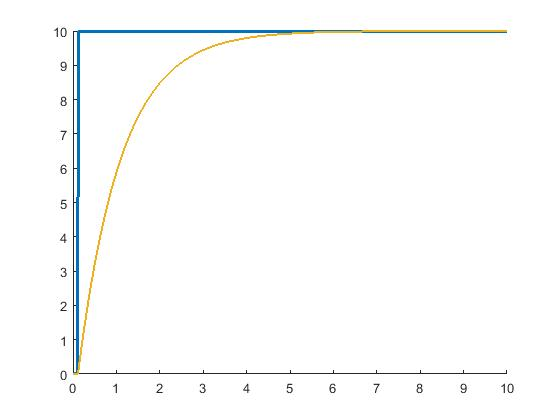
\includegraphics[scale=0.75]{rc}
\end{center}
\pagebreak
\subsection{Circuito RL em série}
  Circuito RL\\
  V0100 1 0 PULSE 0 10 0.1 0 0 2 3 2\\
  R0102 2 0 1\\
  L0102 1 2 1\\
  .TRAN 10 0.01 TRAP 1\\

  \begin{center}
  \hspace*{-2.5cm}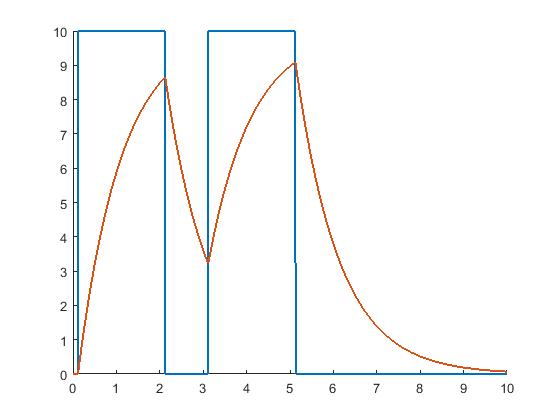
\includegraphics[scale=0.75]{rl}
  \end{center}
\pagebreak
\subsection{Transformador com fonte senoidal}
  TRANSFORMADOR IDEAL
  V 1 0 SIN 0.5 10 1 0 1 0 4\\
  K 1 0 3 0 2\\
  R1 3 0 1\\
  .TRAN 5 0.1 TRAP 4\\

  \begin{center}
  \hspace*{-5cm}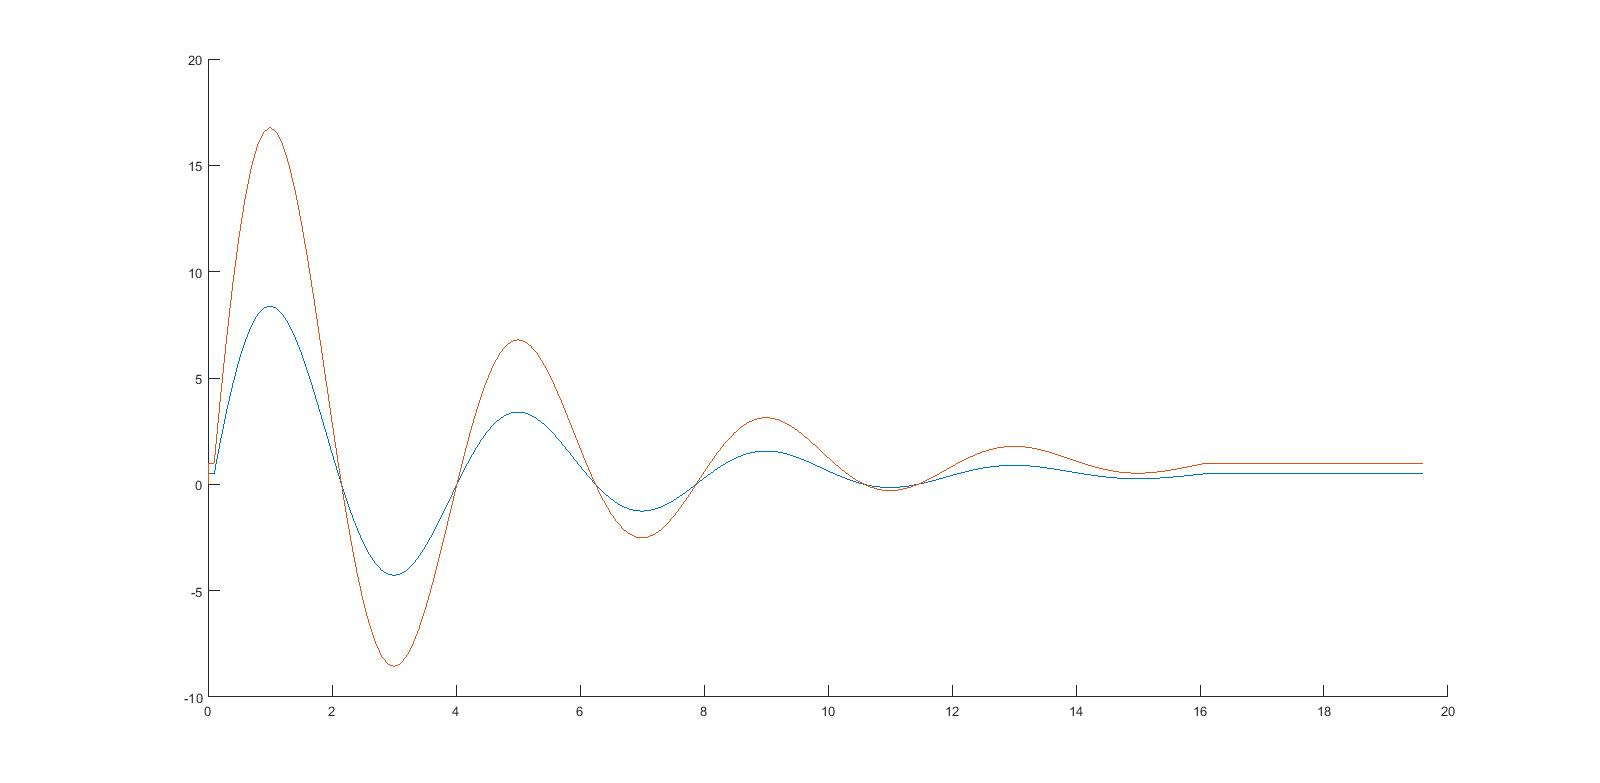
\includegraphics[scale=0.4]{transformador}
  \end{center}
\pagebreak
\subsection{Fonte retificada com filtro capacitivo (tap central simulado por duas fontes)}
  Fonte regulada com filtro capacitivo\\
  V1 1 0 SIN 0 12 60 0 0 0 100000\\
  V2 0 2 SIN 0 12 60 0 0 0 100000\\
  D1 1 3\\
  D2 2 3\\
  C1 3 0 0.2\\
  RL 3 0 1\\
  .TRAN 2 0.00001 TRAP 1\\

  \begin{center}
  \hspace*{-2.5cm}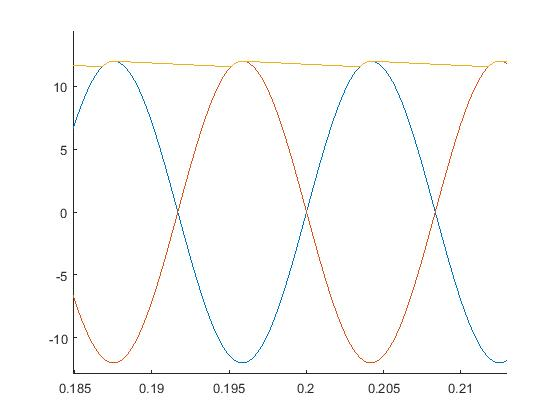
\includegraphics[scale=0.75]{fonteCapacitor}
  \end{center}
\pagebreak
\subsection{Integrador não inversor com amplificadores operacionais}
  CIRCUITO COM  AMPOPS INTERCONECTADOS\\
  R1 1 2 1\\
  C1 2 3 1\\
  O1 3 0 0 2\\
  O2 4 0 4 3\\
  R2 4 5 1\\
  O3 6 0 0 5\\
  R3 5 6 1\\
  V1 1 0 PULSE 0 10 0.01 0 0 100 101 1\\
  .TRAN 10 0.01 TRAP 1\\
  \begin{center}
  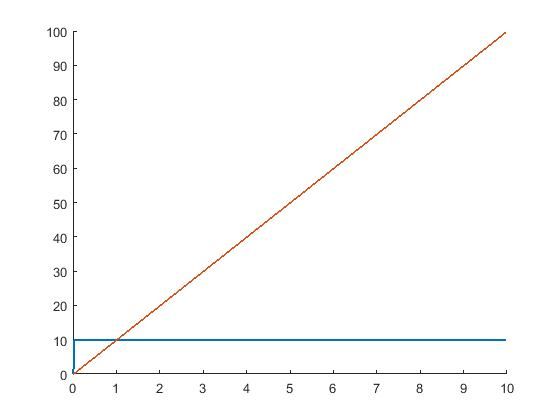
\includegraphics[scale=0.75]{ampops}
  \end{center}

\end{document}
